\section{Retrieval-Augmented Generation}

\subsection{Tổng quan về RAG}
Mô hình ngôn ngữ lớn như GPT, BART hay T5 dù có khả năng biểu diễn ngôn ngữ phong phú, vẫn đối mặt với các hạn chế cơ bản: (i) tri thức nội tại bị giới hạn theo thời điểm cắt dữ liệu huấn luyện, và (ii) hiện tượng hallucination, tức là mô hình sinh ra thông tin sai lệch hoặc không được kiểm chứng một cách tự tin nhưng vô căn cứ \cite{turn0search31, turn0academia26, turn0search0}.  

RAG được đề xuất nhằm kết hợp khả năng sinh ngôn của LLMs với cơ chế truy xuất thông tin từ nguồn tri thức ngoại bộ, giúp nâng cao độ chính xác và cập nhật tri thức mà không cần tái huấn luyện mô hình \cite{lewis2020rag, turn0search27}. RAG hoạt động bằng cách truy xuất các đoạn văn bản liên quan từ kho ngữ liệu ngoài (ví dụ: cơ sở dữ liệu embedding) và dùng chúng làm ngữ cảnh bổ sung cho mô hình sinh, qua đó giảm thiểu hallucination và mở rộng phạm vi tri thức vượt qua giới hạn tri thức nội tại của LLMs \cite{turn0search27, turn0academia24}.

Các kết quả khảo sát gần đây cũng chỉ ra rằng RAG là một thành phần trung tâm trong các hệ thống NLP hiện đại, đồng thời mở ra các hướng mở rộng như GraphRAG để xử lý các mối quan hệ phức tạp hơn trong dữ liệu \cite{turn0search0, turn0search2}. Tiếp nối thành tựu này, các phương pháp như Fusion-in-Decoder đã được phát triển nhằm cải thiện cách tích hợp thông tin truy xuất vào quá trình sinh \cite{izacard2021fid}.

\subsection{Kiến trúc và cơ chế hoạt động của RAG}
\label{sec:rag_arch}
Kiến trúc RAG tiêu chuẩn gồm hai thành phần chính: \textbf{Retriever} và \textbf{Generator}. Quy trình điển hình diễn ra theo ba bước: (1) mã hóa truy vấn và truy xuất \(k\) tài liệu liên quan, (2) kết hợp các tài liệu đó với truy vấn gốc, và (3) sinh câu trả lời dựa trên ngữ cảnh tổng hợp \cite{lewis2020rag, turn0search27}.

\paragraph{Retriever ($p_\eta(z|x)$):}  
Thành phần này chịu trách nhiệm định vị các đoạn văn bản phù hợp nhất từ kho dữ liệu. Các hệ thống hiện đại thường sử dụng Dense Retrieval với mô hình Bi-Encoder, trong đó truy vấn \(x\) và tài liệu \(z\) được ánh xạ thành vector embedding; các vector này sau đó được so sánh để tìm tài liệu liên quan nhất \cite{karpukhin2020dpr}. Phép tìm kiếm tương đồng được thực hiện thông qua cấu trúc như MIPS trong các thư viện như FAISS.

\begin{figure}
    \centering
    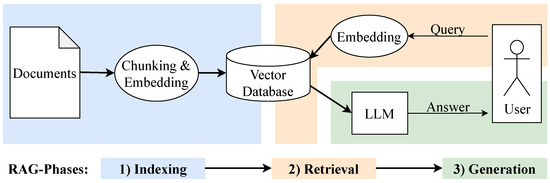
\includegraphics[width=0.75\linewidth]{rag.png}
    \caption{Kiến trúc hệ thống RAG đơn giản.}
    \label{fig:rag_arch}
\end{figure}

\paragraph{Generator ($p_\theta(y|x, z)$):}  
Generator là mô hình sinh câu trả lời dựa trên truy vấn và các đoạn văn bản đã truy xuất. Thường là mô hình seq2seq (như BART, T5) với hai chiến lược fusion chính:  
\begin{itemize}
    \item \textbf{Late Fusion (RAG-Token):} Mỗi tài liệu truy xuất sinh ra phân phối xác suất từ vựng riêng và sau đó được tổng hợp thông qua marginalization \cite{lewis2020rag}.  
    \item \textbf{Early Fusion (Fusion-in-Decoder – FiD):} Các đoạn văn bản được xử lý độc lập ở encoder nhưng được đưa đồng thời vào decoder, cho phép cơ chế attention bao quát toàn bộ ngữ cảnh \cite{izacard2021fid}.
\end{itemize}

\paragraph{Indexing:}  
Dữ liệu nguồn được chunking thành các đoạn văn (ví dụ: 300–500 tokens) và chuyển sang vector embedding để indexing. Khi kiến thức mới xuất hiện, chỉ mục vector có thể được cập nhật độc lập mà không cần thay đổi trọng số của mô hình sinh, tạo thuận lợi cho cập nhật tri thức một cách linh hoạt \cite{lewis2020rag}.

\subsection{Thách thức của RAG}
Mặc dù RAG cải thiện đáng kể hiệu suất và tính tin cậy so với LLM thuần túy, việc triển khai trong các bài toán phức tạp như hỏi–đáp lịch sử hay pháp lý vẫn gặp nhiều thách thức:

\begin{itemize}
    \item \textbf{Sai số truy xuất:} Chất lượng câu trả lời phụ thuộc vào chất lượng các tài liệu được truy xuất; các truy vấn mơ hồ có thể trả về thông tin nhiễu, dẫn tới câu trả lời sai lệch \cite{turn0search27}.
    \item \textbf{Mất ngữ cảnh toàn cục:} Chunking tài liệu có thể làm mất liên kết bối cảnh rộng hơn, ảnh hưởng đến tính mạch lạc của câu trả lời \cite{turn0search1, turn0search0}.
    \item \textbf{Hạn chế suy luận đa bước:} RAG cơ bản gặp khó khăn khi kết nối các mảnh thông tin rời rạc không nằm trong cùng một đoạn văn \cite{turn0search1, turn0search27}.
    \item \textbf{Tính minh bạch:} Dù RAG có thể cung cấp trích dẫn văn bản, việc giải thích quy trình tổng hợp thông tin trong mô hình sinh và đánh giá độ tin cậy vẫn là thách thức nghiên cứu mở \cite{turn0search27}.
\end{itemize}

Những hạn chế này, đặc biệt về suy luận phức tạp và biểu diễn tri thức cấu trúc, là động lực thúc đẩy các phương pháp mở rộng như GraphRAG, trong đó Knowledge Graph được tích hợp để nâng cao hiệu quả truy xuất và kết nối tri thức phức tạp \cite{turn0search1, turn0search0}.